\documentclass[10pt,a4paper]{article}
\usepackage{graphicx}
\usepackage{listings}
\begin{document}
\title{Exponential function: Quick and Dirty}
\author{Martin Cradock Østerlund}
\maketitle

\begin{abstract}
    The exponential function is a very important function used in multiple fields in physics. This short paper introduces a 
    numerical computation of the exponential function, which uses only multiplication and division. I will be comparing it to 
    the exponential algorithm implemented in C\#. 
\end{abstract}

\section{Introduction}
    The "Quick and Dirty" implementation we will be looking at goes as follows.
    \begin{verbatim}
    static double ex(double x){
        if(x<0)return 1/ex(-x);
        if(x>1.0/8) return Pow(ex(x/2),2);
        return 1+x*(1+x/2*(1+x/3*(1+x/4*(1+x/5*(1+x/6*(1+x/7*(1+x/8*(1+x/9*(1+x/10)))))))));
    }
    \end{verbatim}

    This implementation writes the exponential function as its Taylor series, including the first 10 elements of the series. If 
    the function recieves a negative value, it calls the function as $exp(-x)^{-1}$. If we supply a value that is lower than some certain
    precision, in this case $1/8$, the function is called recursively as $exp(x/2)^{2}$ in order to get the required precision. In figure 
    \ref{fig1}, the comparison between the "Quick and Dirty" implementation and the actual exponential function is shown.

    \begin{figure}
        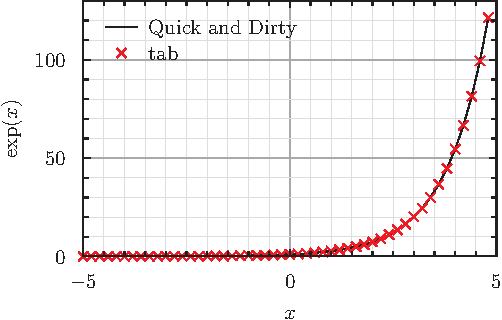
\includegraphics{exp_pyxplot.pdf}
        \caption{The comparison between the exponential function and the "Quick and Dirty" implementation.}
        \label{fig1}
    \end{figure}
    

\end{document}
    